\documentclass[10pt, conference]{IEEEtran}
\usepackage{cite}
\usepackage{amsmath,amssymb,amsfonts}
\usepackage{graphicx}
\usepackage{xcolor}
\usepackage{booktabs}
\usepackage{tikz}
\graphicspath{{../results/}}
\usetikzlibrary{arrows.meta,positioning,calc}
\usepackage[hidelinks]{hyperref}
\newcommand{\todo}[1]{\textcolor{red}{[#1]}}

\begin{document}
\title{Predictive Tracking and Elevation Control for the Mumbai 2044 Guardian Point-Defense Turret:\\
Delay-Matched Type-1 Compensation with a Variable-Step Kalman Predictor}

\author{\IEEEauthorblockN{\todo{Team member names, roll numbers}}
\IEEEauthorblockA{ME319: Control Systems, Dept.\ of Mechanical Engineering, IIT Bombay, Mumbai, India\\
Code: \url{https://github.com/YOUR-USERNAME/YOUR-REPO} \todo{replace}}}
\maketitle

\begin{abstract}
A predictive-feedback fire-control system is designed for the elevation axis of a laser turret engaging a maneuvering aerial target from noisy 20\,Hz range/bearing radar with temporary dropouts. A six-state constant-acceleration Kalman filter with variable-step prediction, and a closed-form $t_p=0.5$\,s extrapolation, supply an elevation reference. The central design idea is that the hit criterion is evaluated against the \emph{current} target position while the reference is the \emph{future} one; hence a type-1 loop whose ramp lag $1/K_v$ equals $t_p$ makes the turret point at the target at the instant of firing. This is achieved with a single gain $K_p=2000$\,V/rad ($\omega_{gc}=2.00$\,rad/s, PM $=89.6^\circ$, GM $=14.4$\,dB). A firing supervisor issues clean single-step pulses. With the turret starting \emph{unaligned} at $0^\circ$, all pulses hit in scenarios A--C (first hit 3.2--3.8\,s, worst pulse miss 1.45\,m) and a 200-case Monte Carlo study over random admissible maneuvers and blackouts gave a 100\% interception rate (median first hit 3.65\,s).
\end{abstract}
\begin{IEEEkeywords}
Kalman filtering, target prediction, fire control, delay matching, turret control, measurement loss.
\end{IEEEkeywords}

%=====================================================================
\section{Introduction}
Gun and laser fire control has always required directing the weapon at the target's future position. In this work the elevation axis of the Guardian turret must track a V-44 target using only noisy range $r$ and elevation $\theta$ at 20\,Hz ($\sigma_r=1$\,m, $\sigma_\theta=0.02^\circ$), with possible radar blackouts $t_{bo}\le0.5$\,s starting at $t\ge1$\,s, a prediction horizon $t_p=0.5$\,s, hard stops $-10^\circ\le\theta\le85^\circ$, and a laser recharge time of 1\,s. A pulse hits if the beam passes within $R_{eng}=2$\,m of the target.

\textbf{Objectives.} (i) Estimate target motion from $(r,\theta)$; (ii) predict the position at $t+t_p$ and convert it to an elevation reference; (iii) design an LTI compensator $G_c(s)$ for the derived plant; (iv) fire only when the beam is aligned. The estimator, predictor and controller are designed once and are \emph{not} retuned per scenario.

\textbf{Design approach and key insight.} Because laser propagation is instantaneous, the beam must intersect the target's \emph{current} position at the firing instant. Aiming the \emph{reference} at the future position $t_p$ ahead is therefore only correct if the closed loop itself delays the reference by about $t_p$. A type-1 loop does this naturally (Section~\ref{sec:ctrl}); a type-2 PI/PID loop, in contrast, tracks ramps with zero lag and would place the beam a distance $\approx r\,\dot\theta_{LOS}\,t_p$ ahead of the target (about 29\,m for the nominal trajectory). The lag is thus used as a design variable rather than minimized. Established tools (CA Kalman filter, polynomial extrapolation) are treated as prior art; the contribution is their adaptation: variable-step filtering robust to dropouts, delay-matched compensation, and alignment-based firing logic.

%=====================================================================
\section{System Architecture}
Fig.~\ref{fig:arch} shows the information flow. The radar gives $(r_m,\theta_m)$ and a validity flag; measurements are converted to Cartesian form and fused by the Kalman filter; the estimate is extrapolated to $t+t_p$ to form $\theta_{ref}$; a P compensator with voltage saturation drives the motor--gear--turret plant; the firing supervisor compares the estimated line of sight with the turret axis.

\begin{figure}[t]
\centering
\resizebox{\columnwidth}{!}{%
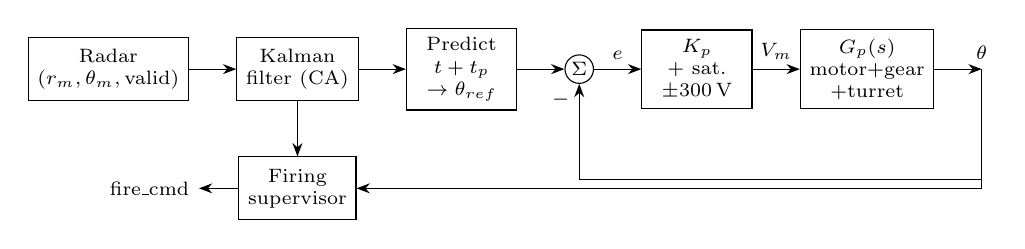
\begin{tikzpicture}[>=Stealth, node distance=7mm and 6mm,
 blk/.style={draw, rectangle, minimum height=8mm, minimum width=14mm, align=center, font=\scriptsize},
 sm/.style={circle, draw, inner sep=1pt, font=\scriptsize}]
\node[blk] (rad) {Radar\\$(r_m,\theta_m,\text{valid})$};
\node[blk, right=of rad] (kf) {Kalman\\filter (CA)};
\node[blk, right=of kf] (pr) {Predict\\$t+t_p$\\$\to\theta_{ref}$};
\node[sm, right=of pr] (sum) {$\Sigma$};
\node[blk, right=of sum] (gc) {$K_p$\\+ sat.\\$\pm300$\,V};
\node[blk, right=of gc] (gp) {$G_p(s)$\\motor+gear\\+turret};
\node[blk, below=7mm of kf] (fire) {Firing\\supervisor};
\draw[->] (rad)--(kf); \draw[->] (kf)--(pr); \draw[->] (pr)--(sum);
\draw[->] (sum)--node[above,font=\scriptsize]{$e$}(gc);
\draw[->] (gc)--node[above,font=\scriptsize]{$V_m$}(gp);
\draw[->] (gp.east)--++(6mm,0) coordinate(o) node[above,font=\scriptsize]{$\theta$};
\draw[->] (o)--++(0,-14mm)-|(sum) node[pos=0.92,left,font=\scriptsize]{$-$};
\draw[->] (kf)--(fire); \draw[->] (o)|-(fire);
\draw[->] (fire.west)--++(-5mm,0) node[left,font=\scriptsize]{fire\_cmd};
\end{tikzpicture}}
\caption{Predictive-feedback architecture.}\label{fig:arch}
\end{figure}

\begin{figure}[t]
\centering
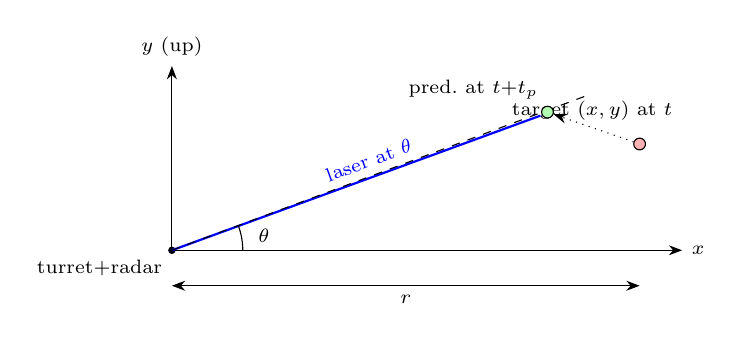
\begin{tikzpicture}[>=Stealth, scale=0.9, font=\scriptsize]
\draw[->] (0,0)--(7.2,0) node[right]{$x$}; \draw[->] (0,0)--(0,2.6) node[above]{$y$ (up)};
\fill (0,0) circle (1.5pt) node[below left]{turret+radar};
\draw[thick,blue] (0,0)--(5.2,1.9) node[pos=0.55,above,sloped]{laser at $\theta$};
\draw[dashed] (0,0)--(5.9,2.2);
\node[draw,circle,inner sep=1.5pt,fill=red!30] (c) at (6.6,1.5) {};
\node[above left] at (7.2,1.7) {target $(x,y)$ at $t$};
\node[draw,circle,inner sep=1.5pt,fill=green!30] (p) at (5.3,1.95) {};
\node[above left] at (5.3,2.0) {pred.\ at $t{+}t_p$};
\draw[->,dotted] (c)--(p);
\draw (1.0,0) arc (0:20:1.0); \node at (1.3,0.2) {$\theta$};
\draw[<->] (0,-0.5)--node[below]{$r$}(6.6,-0.5);
\end{tikzpicture}
\caption{Elevation-plane geometry: turret and radar co-located at the origin; the turret is commanded to the predicted line of sight.}\label{fig:geom}
\end{figure}

%=====================================================================
\section{Mathematical Modeling}
\subsection{Turret elevation plant}
Assumptions: rigid gear train (no backlash), constant parameters, $J_m$ reflected through $N$, turret-side viscous friction $b$, no gravity or payload imbalance (elevation torque from gravity omitted), and motion away from the hard stops (the model is linear there). With $\omega_m=N\dot\theta$, the armature loop and the reflected mechanics are
\begin{align}
L_m \dot i + R_m i + N K_e\dot\theta &= V_m,\\
J_{eq}\ddot\theta + b\dot\theta &= N K_t i,
\end{align}
with $J_{eq}=J_t+N^2J_m=3200$\,kg\,m$^2$.
With state $[\theta\ \dot\theta\ i]^T$ and input $V_m$:
\begin{equation}\scriptsize
\begin{split}G_p(s)&=\frac{N K_t}{J_{eq}L_m s^3+(J_{eq}R_m{+}bL_m)s^2+(bR_m{+}N^2K_tK_e)s}\\
&=\frac{1000}{320s^3+3350s^2+1.0015{\times}10^6 s}\end{split}
\end{equation}
Poles: $s=0$ and $s=-5.23\pm j55.70$ ($\omega_n=55.9$\,rad/s, $\zeta=0.094$): a lightly damped electromechanical resonance that bounds the usable bandwidth. The low-frequency behavior is $G_p(s)\approx 1/(1001.5\,s)$, i.e.\ a velocity gain $K_{dc}=N K_t/(bR_m+N^2K_tK_e)=9.985{\times}10^{-4}$\,rad/s per V; the 3.35\,ms electrical/inertial lag is negligible at the closed-loop bandwidth.

\subsection{Target-state estimation}
Polar measurements are converted to Cartesian, $z=[r_m\cos\theta_m,\ r_m\sin\theta_m]^T$, so the process model stays linear. The state is $\mathbf{x}=[x\ \dot x\ \ddot x\ y\ \dot y\ \ddot y]^T$ with constant-acceleration kinematics driven by white jerk:
\begin{align}
\mathbf{F}(\Delta)&=\text{blkdiag}(F_1,F_1),\ F_1=\begin{bmatrix}1&\Delta&\Delta^2/2\\0&1&\Delta\\0&0&1\end{bmatrix},\\
Q_1(\Delta)&=q\begin{bmatrix}\Delta^5/20&\Delta^4/8&\Delta^3/6\\ \Delta^4/8&\Delta^3/3&\Delta^2/2\\ \Delta^3/6&\Delta^2/2&\Delta\end{bmatrix},
\end{align}
with $\mathbf Q=\text{blkdiag}(Q_1,Q_1)$ and $q=50$\,m$^2$/s$^5$ (the standard maneuver jerks of 8--12\,m/s$^3$ in scenario B motivated this order of magnitude; a CV model cannot follow accelerating targets and an overly large $q$ amplifies noise). $\Delta$ is the \emph{actual} time since the last accepted measurement, so a blackout is simply a longer prediction step with correspondingly larger covariance growth, with no special mode. The measurement covariance is the linearized polar-to-Cartesian map
\begin{equation}\small
R=\begin{bmatrix}\sigma_r^2c^2{+}r^2\sigma_\theta^2s^2&(\sigma_r^2{-}r^2\sigma_\theta^2)cs\\ \cdot&\sigma_r^2s^2{+}r^2\sigma_\theta^2c^2\end{bmatrix},
\end{equation}
($c=\cos\theta_m$, $s=\sin\theta_m$). At 1500\,m, $r\sigma_\theta\approx0.52$\,m, so range and cross-range errors are comparable and the rotation matters. The filter is initialized from the first measurement with $P_0=\text{diag}(4,75^2,15^2)$ per axis, reflecting only the bounds $|v|\le150$, $|a|\le20$ (no knowledge of the true velocity). The update uses the Joseph form. A measurement is accepted only if \texttt{meas\_valid}$=1$ and at least $T_s=50$\,ms has elapsed, which makes the filter independent of the simulator step.

\subsection{Prediction and elevation reference}
Between updates the state is extrapolated by $\delta=t-t_k$, and the prediction horizon is $\delta+t_p$:
\begin{align}
\hat p(t{+}t_p)&=\hat p_k+\hat v_k(\delta+t_p)+\tfrac12\hat a_k(\delta+t_p)^2,\ p\in\{x,y\},\\
\theta_{ref}&=\text{sat}_{[-10^\circ,85^\circ]}\,\text{atan2}(\hat y(t{+}t_p),\hat x(t{+}t_p)).
\end{align}
The second-order extrapolation is exact for constant acceleration; its error under jerk $j$ is $\tfrac16 j\,t_p^3$ per axis, e.g.\ 0.2\,m for $j=10$\,m/s$^3$ at $t_p=0.5$\,s, negligible compared with filter noise.

%=====================================================================
\section{Controller Design and Analysis}\label{sec:ctrl}
\subsection{Delay-matching design}
Let $L(s)=K_pG_p(s)$ and $T=L/(1+L)$. For low frequencies, $L\approx K_v/s$ with $K_v=K_pK_{dc}$ and $T\approx 1/(1+s/K_v)\approx e^{-s/K_v}$, i.e.\ a lag of $1/K_v$. The hit condition requires $\theta(t)\approx\theta_{LOS}(t)=\theta_{ref}(t-t_p)$ since $\theta_{ref}(t)=\theta_{LOS}(t+t_p)$. Hence
\begin{equation}
\frac1{K_v}=t_p\ \Rightarrow\ K_p=\frac{1}{t_pK_{dc}}\approx2005\ \to\ 2000\ \text{V/rad}.
\end{equation}
The residual mismatch between the first-order lag and the pure delay is $T e^{t_ps}-1\approx\tfrac12t_p^2s^2$, giving a tracking error $e_\theta\approx\tfrac18\ddot\theta_{LOS}$. For scenario B ($|\ddot\theta_{LOS}|\approx a_\perp/r\approx7{\times}10^{-3}$\,rad/s$^2$ at $\sim$1500\,m) this is $\sim$0.9\,mrad, i.e.\ $\sim$1.3\,m at 1500\,m, within $R_{eng}$ before filter error. 

\textbf{Why not PI/PID.} Adding integral action raises the system type to 2 and removes the ramp lag. The turret would then lead the target by $t_p$ (miss $\approx r\,\dot\theta_{LOS}\,t_p\approx$ 29\,m, nominal), so a PI/PID loop fails the hit criterion on constant-velocity targets once it has converged, even though its tracking of $\theta_{ref}$ is excellent. Derivative action is also unnecessary: the loop crosses over two decades below the resonance, and omitting $K_d$ avoids differentiating the noisy reference.

\subsection{Frequency-domain verification}
Table~\ref{tab:margins} lists the exact values for $L(s)=2000\,G_p(s)$ (computed numerically).
\begin{table}[t]
\caption{Loop and closed-loop characteristics ($K_p=2000$)}\label{tab:margins}
\centering\small
\begin{tabular}{lc}
\toprule
Gain crossover $\omega_{gc}$ & 2.00 rad/s\\
Phase margin & $89.6^\circ$\\
Phase crossover / gain margin & 55.9 rad/s / 14.4 dB\\
Velocity constant $K_v$ / lag $1/K_v$ & 1.997 s$^{-1}$ / 0.501 s\\
Closed-loop poles & $-2.01$; $-4.23\pm j55.6$\\
Closed-loop $-3$\,dB bandwidth & 2.01 rad/s\\
Step overshoot / 2\% settling & $\approx0$ / 1.95 s\\
\bottomrule
\end{tabular}
\end{table}
The dominant pole at $-2.01$ (time constant 0.50\,s) gives a monotone, non-overshooting response; the lightly damped pair ($\zeta\approx0.076$) is only weakly excited because the loop gain at $\omega_n$ is small. The gain margin limits $K_p\lesssim10\,400$ V/rad, so the design sits a factor 5.2 below instability and is robust to $\pm$ parameter errors (e.g., a 30\% error in $b$ or $K_t$ changes $K_v$ and hence the lag, but not stability).

\subsection{Noise, saturation, hard stops, measurement loss}
\emph{Noise:} the controller is a pure gain, so reference noise reaches $V_m$ scaled by only $K_p$, then low-pass filtered by the plant ($\omega_{bw}\approx2$\,rad/s). \emph{Saturation:} steady tracking requires $V\approx\dot\theta_{LOS}/K_{dc}$ plus a small acceleration term: $\approx40$--60\,V for the scenarios (Fig.~\ref{fig:scen}), far below 300\,V. Saturation occurs only in the initial slew from a large initial error ($\approx8\%$ of the run), where the absence of an integrator means no windup can occur. \emph{Hard stops:} references are clipped to $[-10^\circ,85^\circ]$ and the simulator zeroes the turret velocity state at a stop. \emph{Measurement loss:} the filter propagates with CA kinematics; position uncertainty after a gap $\Delta$ grows roughly as $\tfrac12\sigma_a\Delta^2$ with $\sigma_a$ the acceleration uncertainty, and the reference extrapolates over up to $\Delta+t_p=1$\,s. The error is bounded by the physical acceleration limit (20\,m/s$^2$ $\Rightarrow$ $\le$10\,m, 7\,mrad, in the worst case at 1\,s), so blackouts are the main source of prediction error; because the supervisor fires only when the \emph{estimated} miss is small, the effect is delayed or skipped pulses rather than wild shots.

\subsection{Firing supervisor}
With estimated current target $(\hat x_n,\hat y_n)$ and turret angle $\theta$, the beam miss is $d=|\hat x_n\sin\theta-\hat y_n\cos\theta|$ with $\hat x_n\cos\theta+\hat y_n\sin\theta>0$. A pulse is issued when $d\le1$\,m (half of $R_{eng}$, leaving room for $\sim$0.5\,m estimation error), at least 8 measurements ($0.4$\,s) have been fused, and $\ge1$\,s has elapsed since the last pulse. \texttt{fire\_cmd} is high for a single step, so each pulse is a clean $0\to1$ edge, and repeats every 1\,s while aligned, which also improves consistency across cases.

%=====================================================================
\section{Simulation and Results}
\textbf{Setup.} Plant integrated with RK4, $\Delta t=5$\,ms, $0\le t\le10$\,s, seed 42, using the specified parameters and functions. The turret starts at $0^\circ$ (the target LOS starts at $\approx19.6^\circ$), i.e.\ deliberately \emph{not} aligned. Design parameters: $K_p=2000$, $q=50$, $P_0$ as above, $T_s=50$\,ms, gate 1\,m, minimum 8 updates. Miss distance uses the true target position at the pulse instant.

\begin{table}[t]
\caption{Standard scenarios (single design, turret start $0^\circ$)}\label{tab:res}
\centering\small
\begin{tabular}{@{}l@{\ }c@{\ }c@{\ }c@{\ }c@{\ }c@{}}
\toprule
Scen. & Pulses & Hits & 1st hit [s] & Min [m] & Max [m]\\
\midrule
A & 7 & 7 & 3.16 & 0.23 & 1.15\\
B & 6 & 6 & 3.50 & 0.21 & 1.45\\
C & 6 & 6 & 3.81 & 0.26 & 1.14\\
\bottomrule
\end{tabular}
\end{table}

\begin{figure}[t]
\centering
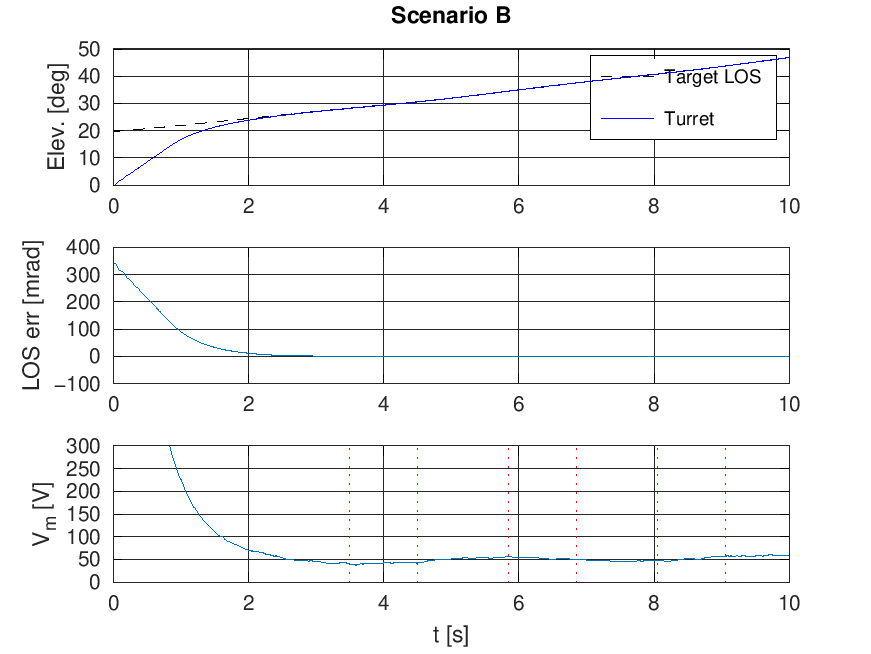
\includegraphics[width=0.95\columnwidth]{scenario_B.png}
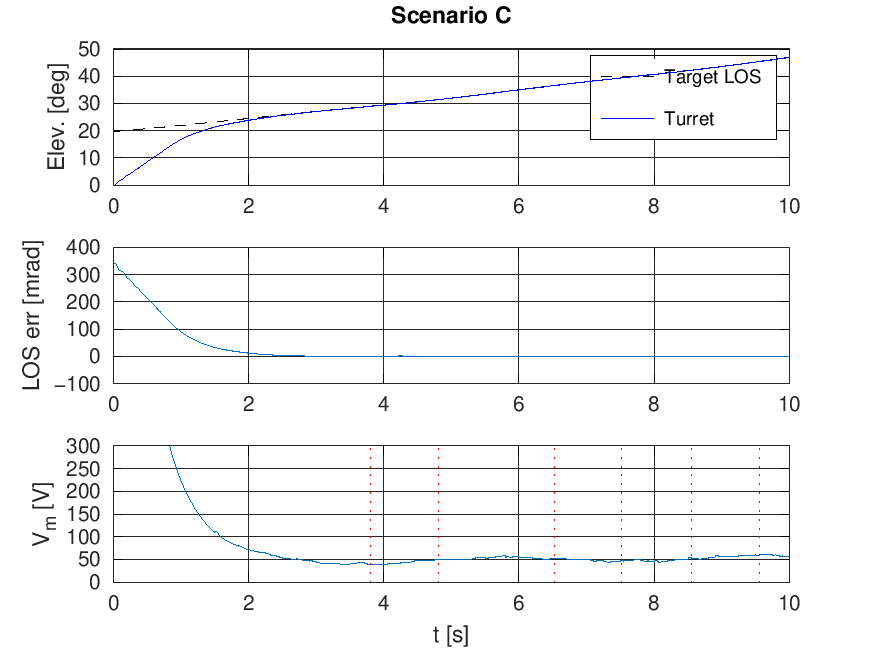
\includegraphics[width=0.95\columnwidth]{scenario_C.png}
\caption{Scenarios B (top) and C (bottom): target LOS vs.\ turret, LOS error, motor voltage (dotted lines: pulses).}\label{fig:scen}
\end{figure}

\textbf{Interpretation.} After the initial slew ($\approx$2--3\,s, set by the 0.5\,s closed-loop time constant and 300\,V saturation) the LOS error is below a few mrad and the steady voltage is about 40--60\,V. First-hit time is therefore dominated by the start transient, not by estimation. In C the blackout ($1.0$--$1.5$\,s) occurs while the turret is still slewing, so the controller is largely unaffected; the later first hit (3.81\,s vs.\ 3.50\,s) reflects the filter's larger covariance after the gap and the 1\,m gate. \todo{Add a figure of estimated vs.\ true position, prediction error and $\mathrm{tr}(P)$ growth during the blackout; generate it from logged filter states.}

\subsection{Generalization (Monte Carlo)}
To avoid tuning to three trajectories, 200 randomized cases were simulated with the same fixed design: random initial range (900--1900\,m) and elevation, speed up to 100\,m/s, a smooth maneuver ($a\le20$\,m/s$^2$, $\omega\in[0.5,3]$\,rad/s, onset 1--3\,s), a blackout in 70\% of cases (onset 1--3\,s, duration $\le0.5$\,s), and a random initial turret angle in $[-10^\circ,85^\circ]$. Cases violating range, velocity, acceleration or elevation limits were rejected. Result: \textbf{200/200 intercepted}; first-hit time median 3.65\,s, 90th percentile 5.41\,s, max 8.05\,s; best-pulse miss median 0.13\,m, 90th percentile 0.60\,m; 6.4 pulses per run, all hitting; saturation fraction 11.8\%.

\begin{figure}[t]
\centering
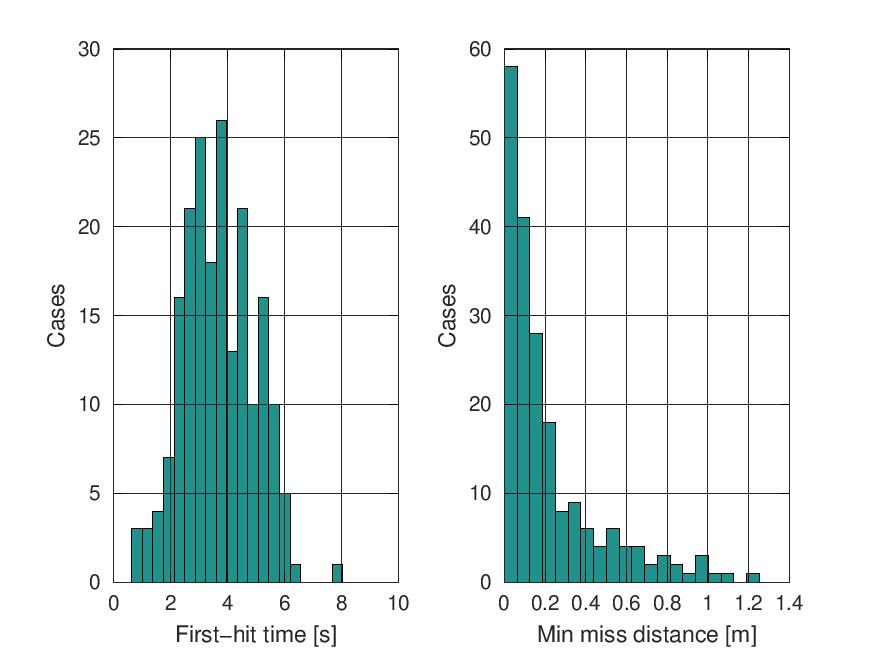
\includegraphics[width=\columnwidth]{mc_hist.png}
\caption{Monte Carlo (200 cases): first-hit time and minimum miss distance.}\label{fig:mc}
\end{figure}

%=====================================================================
\section{Final Evaluation}
\todo{Run the instructor-provided evaluation script with the final \texttt{turret\_controller.m} and report success, interception time, miss distance and consistency across cases here, with a plot. Do not retune afterwards. Replace this note with the actual numbers.}

%=====================================================================
\section{Conclusions}
A delay-matched type-1 loop, $K_p=2000$\,V/rad, turns the lag of the closed loop into a feature: with the reference set $t_p$ ahead, the beam arrives at the current target position. Together with a variable-step CA Kalman filter, it intercepted in all standard and 200 random cases with sub-1.5\,m pulse misses.
\textbf{Strengths:} one design parameter set, analytic gain selection, no noise-amplifying derivative or windup, and robustness to dropouts without special modes.
\textbf{Limitations:} (i) first hit is delayed by the 0.5\,s time constant when the turret starts far from the target, and raising $K_p$ would shorten it at the expense of lag matching; (ii) the lag is matched to one $t_p$ and one $K_{dc}$, so plant parameter variation shifts the aim point proportionally to $r\dot\theta_{LOS}$; (iii) accuracy under strong maneuvers and long dropouts is limited by CA prediction; (iv) gravity, backlash and flexibility are not modeled.

\begin{thebibliography}{00}
\bibitem{b1} R. C. Dorf and R. H. Bishop, \textit{Modern Control Systems}, 13th ed. Pearson, 2017.
\bibitem{b2} Y. Bar-Shalom, X. R. Li, and T. Kirubarajan, \textit{Estimation with Applications to Tracking and Navigation}. Wiley, 2001.
\bibitem{b3} P. Agarwal, ``ME319 Assignment 2: Mumbai 2044,'' IIT Bombay, Autumn 2026.
\end{thebibliography}

%=====================================================================
\clearpage
\section*{Appendix: AI and Computational Tool Documentation}
\small
\textbf{Tools.} \todo{List only what you actually used, e.g.\ Claude (version), ChatGPT, MATLAB/Octave versions, Overleaf.}

\textbf{Contributions.} \todo{Edit to match reality.} An AI assistant reviewed the first-draft code and report, drafted the revised controller, simulation and Monte Carlo scripts, and drafted this LaTeX. MATLAB/Octave executed the simulations.

\begin{table}[h]
\caption{Significant AI/computational outputs and validation}
\centering\scriptsize
\begin{tabular}{p{1.9cm}p{1.0cm}p{4.6cm}}
\toprule
Output & Status & Validation / justification\\
\midrule
Observation that the first design (PID with integral) fires essentially only at $t=0$ when started aligned & Accepted & Reproduced by logging pulse times with an unaligned start; explained by type-2 tracking leading the target by $t_p$ ($\approx$29\,m).\\
Type-1 delay-matched design, $K_p=2000$ & Accepted after checking & $K_v$ and margins recomputed independently (Python/SciPy: $\omega_{gc}=2.00$, PM $89.6^\circ$, GM 14.4\,dB); lag confirmed in simulation.\\
Earlier reported GM of 16.8\,dB for PID & Rejected & Not reproduced by independent frequency-response calculation; replaced by new analysis.\\
Variable-$\Delta$ Kalman filter, jerk-based $Q$ & Modified & $q$ chosen from scenario jerk order of magnitude; \todo{add NIS/NEES consistency check}.\\
Monte Carlo script & Accepted with edits & Random targets verified against range/velocity/acceleration/elevation limits; results tabulated from logs.\\
\bottomrule
\end{tabular}
\end{table}
\textbf{Engineering validation.} Plant transfer function re-derived from Kirchhoff and rotational dynamics; margins and poles computed numerically; simulations checked against hand estimates ($K_v$, steady voltage $\approx\dot\theta_{LOS}/K_{dc}$, error $\approx\tfrac18\ddot\theta_{LOS}$); hard-stop velocity handling and pulse bookkeeping checked in code. \todo{State any further checks you actually performed.}
\end{document}
